\documentclass[french]{article}

\usepackage[french]{babel}

\usepackage[utf8]{inputenc}
\usepackage[T1]{fontenc}
\usepackage[hidelinks]{hyperref}
\usepackage{graphicx}
\usepackage{amsmath}
\usepackage{fullpage}
\usepackage{microtype}
\usepackage{upquote}
\usepackage{listings}
\usepackage{url}
\usepackage[backend=biber]{biblatex}

\usepackage{pdfpages}

\usepackage{titling}
\newcommand{\subtitle}[1]{%
  \posttitle{%
    \par\end{center}
    \begin{center}\large#1\end{center}
    \vskip0.5em}%
}

\addbibresource{references.bib}

\title{Martine résout le problème du voyageur de commerce}
\subtitle{Avec un algorithme A*}
\author{Maxence \textsc{Aïci} \and Rémi \textsc{Nicole}}

\begin{document}

\maketitle

\part{Modélisation}

\paragraph{}
Le problème du voyageur de commerce est probablement le problème NP-complet le
plus connu en algorithmique, mais dans le doute, voici la définition de
Wikipedia~\cite{wiki:tsp}:

\begin{quote}
	``Given a list of cities and the distances between each
	pair of cities, what is the shortest possible route that visits each city
	exactly once and returns to the origin city?''
\end{quote}

\paragraph{}
Quant aux algorithmes de type A*, il s'agit tout simplement d'une amélioration
de l'algorithme de Dijkstra qui choisit sans aucun scrupule les nœuds qui sont
le plus susceptible de nous mener à la solution optimale. On calcule cette
``susceptibilité'' grâce à une heuristique qui calculera de manière arbitraire
une estimation du score restant pour aller à l'arrivée.

De manière mathématique, parce qu'en algorithmie, on aime bien écrire des
équations compliquées, et en plus en \LaTeX, ça nous donne un rendu magnifique:

\[f(n) = g(n) + h(n)\]

Avec:
\begin{itemize}
	\item $n$ l'étape par laquelle l'algorithme suggère de passer
	\item $f(n)$ l'estimation du coût total en passant par l'étape $n$
	\item $g(n)$ le coût d'aller du début jusqu'à l'étape $n$
	\item $h(n)$ l'estimation du coût pour aller de l'étape $n$ à l'arrivée
\end{itemize}

\section{The Problem Solving Graph}

First, we'll define the structure a PSG (Problem Solving Graph) that represents
our progression along the route we are going to take.

If the map of our cities looks like that:
\begin{center}
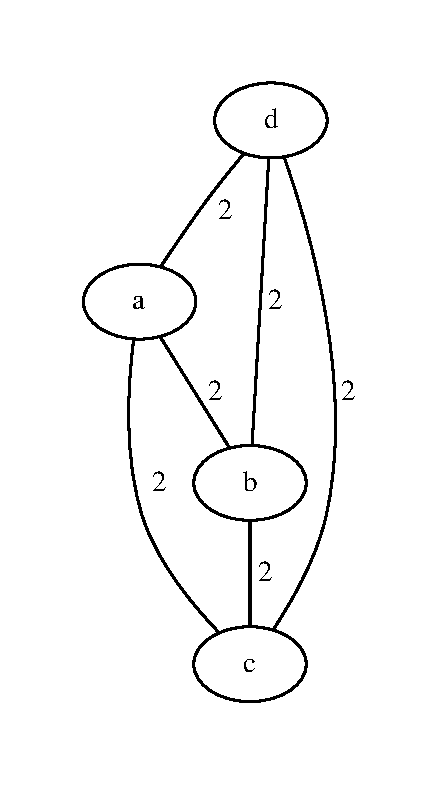
\includegraphics[scale=0.5]{graphs/modeling-the-problem_example1-map.pdf}
\end{center}

The corresponding PSG will be:
\begin{center}
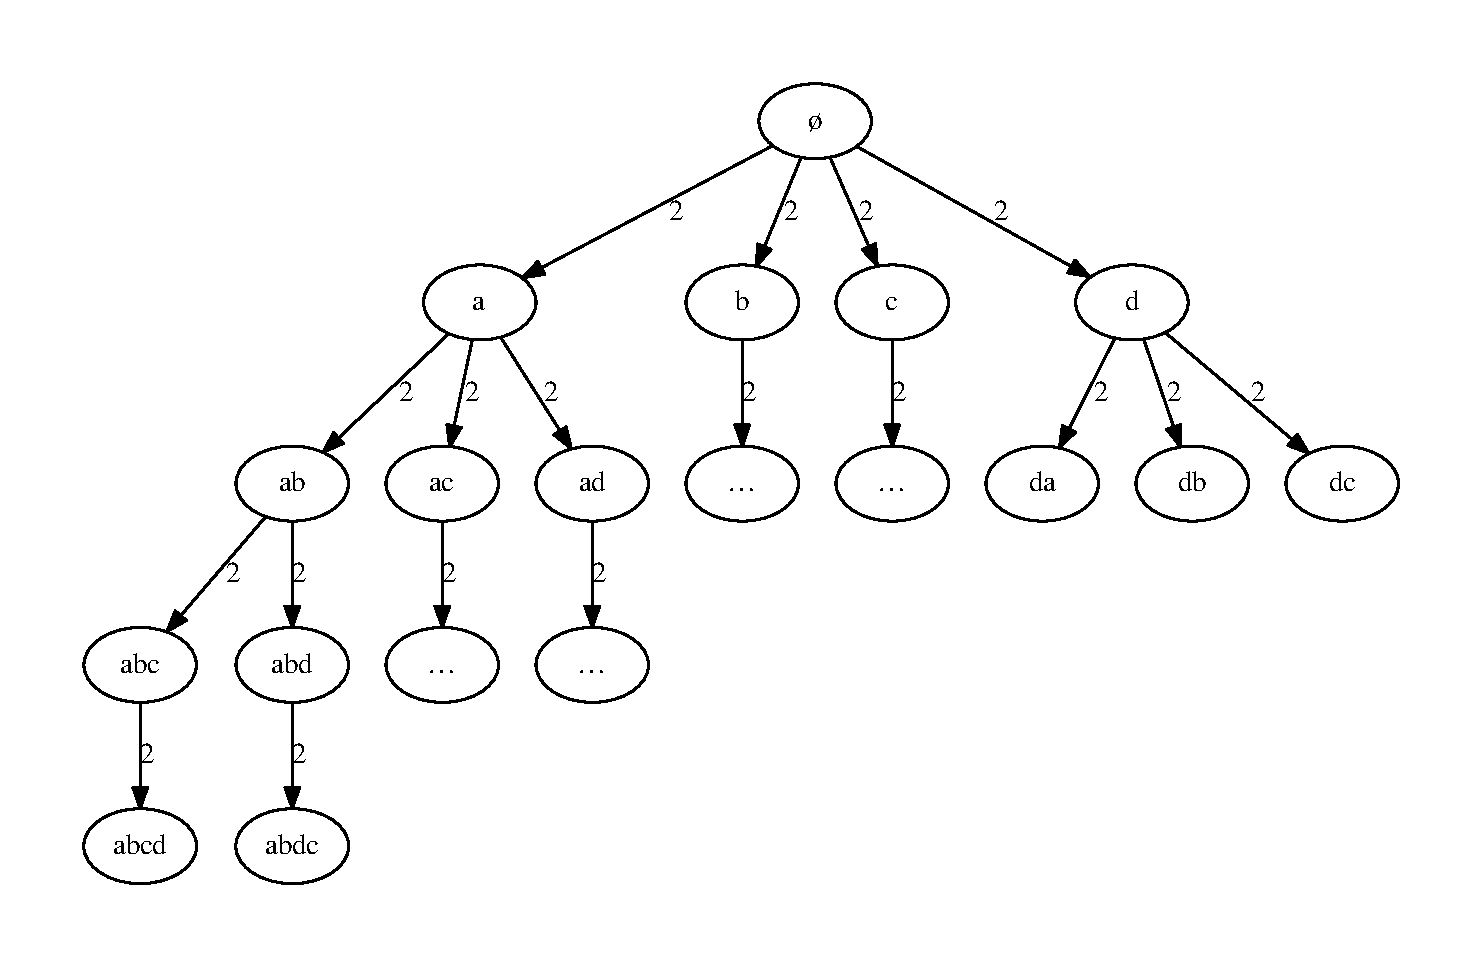
\includegraphics[scale=0.5]{graphs/modeling-the-problem_example1-psg.pdf}
\end{center}

And, for example, after taking the A $\rightarrow$ B $\rightarrow$ C path, we'll have:
\begin{center}
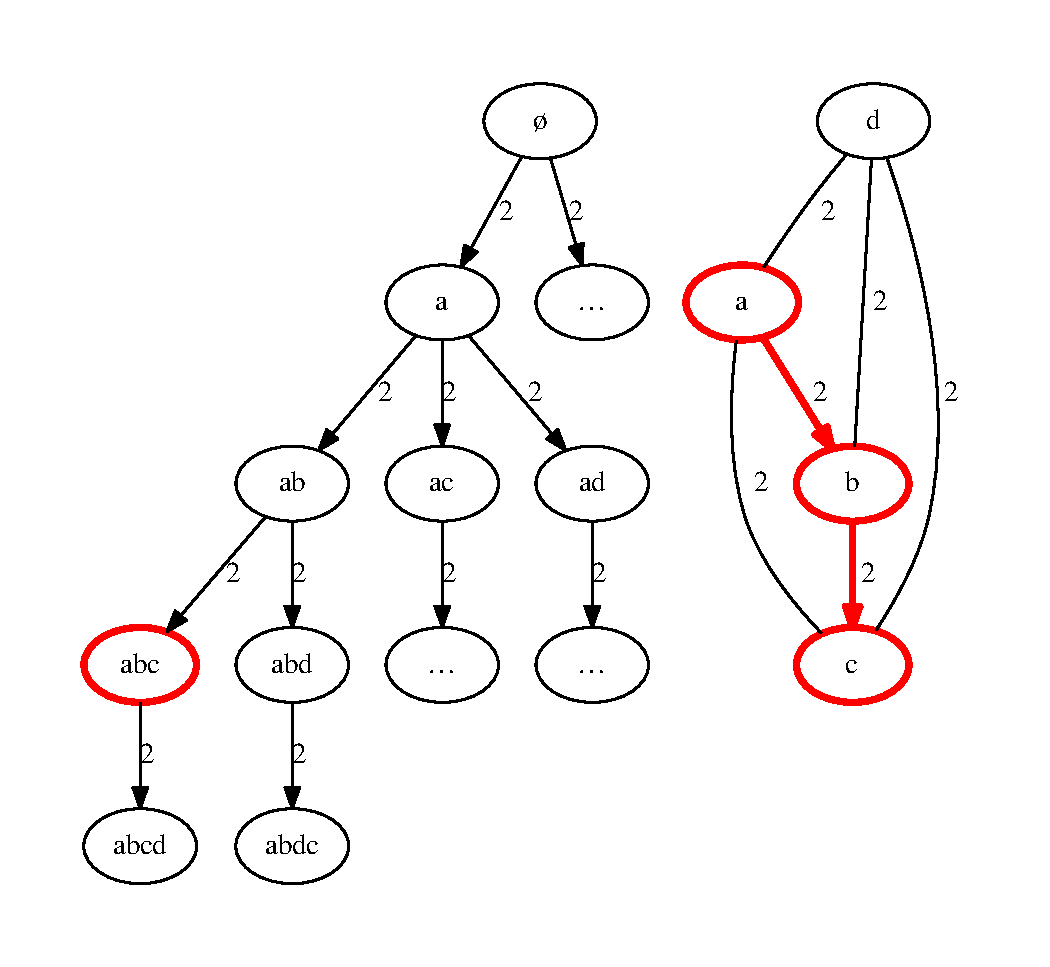
\includegraphics[scale=0.5]{graphs/modeling-the-problem_example2.pdf}
\end{center}

\part{Implementing the data structures}

\printbibliography%

\end{document}
